% Template latex pour des cours ou des petits documents.
% C'est un template pour des cours que j'ai adapté et 
% auquel j'ai ajouté des éléments.
% En cas de problèmes n'hésites pas a me contacter.
% David Tocaven
% david.tocaven@gmail.com

%%% /!\ /!\ /!\ /!\ /!\ /!\
% Se compile avec LaTex et si tu inclus une image matricielle, avec PDFLatex.
%%% /!\ /!\ /!\ /!\ /!\ /!\
\documentclass[12pt]{article}
\usepackage{bbold}
\usepackage{dsfont}
\usepackage[french]{babel}		% Pour avoir le document en français
\usepackage[utf8x]{inputenc}	% Encodage du document
\usepackage{float}				% Pour gérer les positionnement d'images
\usepackage{mathrsfs}			% Pour les lettres calligraphiques équation
\usepackage[colorinlistoftodos]{todonotes}
\usepackage{url}				% Pour faire des hyperliens vers le web
\usepackage{color}
% pour les informations sur un document compilé en PDF et les liens externes / internes
\usepackage{hyperref}			% Pour faire des hyperliens
\usepackage{array}				% Pour faire des tableaux
\usepackage{tabularx}
% pour utiliser 		% floatbarrier
%\usepackage{placeins}
%\usepackage{floatrow}
\usepackage{setspace}			% Espacement entre les lignes
\usepackage{abstract}			% Modifier la mise en page de l'abstract
\usepackage[T1]{fontenc}		% Police et mise en page (marges) du document
\usepackage[top=2cm, bottom=2cm, left=2cm, right=2cm]{geometry}
\usepackage{pdfpages}			% pour inclures des pdf comme des images
\usepackage{subfig}				% Pour les galerie d'images
\usepackage{listings}			% pour inclure du code dans le doc
\usepackage{soul}				% Pour souligner
\usepackage{enumitem}
\usepackage{wrapfig}


\begin{document}
 
% --------------------------------------------------------------
%                         Start here
% --------------------------------------------------------------
 
%\renewcommand{\qedsymbol}{\filledbox}



\title{GitKraken, petit guide}%replace X with the appropriate number
\author{Explications, commandes de bases et scénarios courants} 
\maketitle
\section{Description}
GitKraken est un utilitaire graphique de git, un logiciel de gestion de version de code. Il est possible de lier un code local avec un code stocké en ligne (github dans notre cas) mais ce n'est ni automatique ni obligatoire. C'est ce que l'on appelle une \emph{remote}, qu'il faut initialisée.

Afin de créer un projet, il faut initialiser un versionning.

\section{Commande de base}
Afin de créer un projet, il faut faire des "photos", des versions de l'état du projet à différents moments que l'on choisit en fonction de l'avancement. Quand, au cours du développement, on considère que l'état actuel est intéressant, que l'on pourrait avoir envie d'y retourner, avant de testé quelque choses de nouveau, ... on effectue un \textbf{commit}. Il comprend un titre et une description et le projet à l'état de la création de celui-ci. Les différents \textbf{commits} sont organisés dans des \textbf{branchs}. Celles-ci permettent d'avoir en parallèle différentes versions du code. Il est possible de mettre en ligne avec la commande \textbf{push} la version locale d'une branche. De la même façon, il est possible de récupérer l'état d'une branche depuis internet sur sa version locale avec la commande \textbf{pull}. On peut regrouper deux branches grâce à la commande \textbf{merge}. Pour cela il faut faire glisser la branche cible et la lâcher sur la branche destination. Il faut ensuite choisir \emph{Merge NomBranchCible \textcolor{red}{into}\footnote{À ne pas confondre avec onto.} Merge NomBranchDestination} dans l'onglet déroulant qui apparait . Parfois, la gestion des conflits nécessite un choix qui sera présenté avec un face à face des deux codes. On doit choisir la version a conserver, par bloc de texte modifié ou par ligne.

L'utilisation de branches est très pratique et quasiment indispensable pour travailler à plusieurs sur un même projet. Pour cela, à partir d'un état d'un projet, on crée une branche par fonction et sur celle-ci chaque personne qui intervient crée une branche. Chacun effectue ses modifications et ses \textbf{commits} sur sa branche et la réuni avec develop  quand il le souhaite (le travail est fini, on a besoin d'une version plus récente pour continuer, ...) grâce à la fonction \textbf{merge}. Les branches qui n'ont pas besoin d'être partagées n'ont pas forcément besoin d'être mises en ligne (pas besoin de \emph{push}). 
\newpage
Lorsque l'on travaille à plusieurs sur git (donc avec une version en ligne), il est important de respecter la même organisation :
\begin{figure}[!ht]
\centering
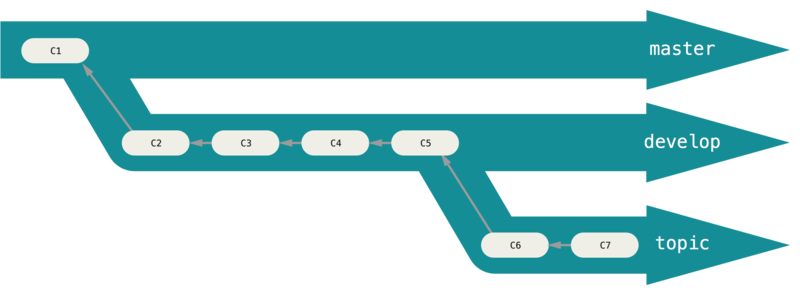
\includegraphics[width=15cm]{./gitSchema.png}
\caption{\label{fig:workflow}WorkFlow d'un projet git}
\end{figure}

Sur la figure \ref{fig:workflow}, la branche \textbf{master} est la branche principale où il ne doit y avoir \ul{que des versions fonctionnelles} du code. A partir de celle-ci, est créer une branche \textbf{develop} où seront fait tous les sous-branchements nécessaires pour faire une nouvelle version fonctionnelle. C'est depuis cette banche que l'on va faire une branche par fonction (\textbf{topics}). \textcolor{red}{Il est nécessaire, avant chaque \textbf{merge}, de \textbf{pull} la branche destination afin d'ajouter nos modifications sur une version à jour de la branche de destination.}

\end{document}